\subsection{Transaction}
\label{sec:transaction}

Trong hệ thống quản lý cơ sở dữ liệu, việc đảm bảo tính toàn vẹn và nhất quán của dữ liệu khi có nhiều thao tác đồng thời là vô cùng quan trọng. Mục này sẽ đi sâu vào cơ chế Transaction trên hai DBMSs: SQL và NoSQL, đồng thời so sánh và áp dụng vào bài toán thực tế.

\subsubsection{Giới thiệu chung về Transaction}
Transaction (Giao dịch) là một chuỗi các thao tác truy xuất hoặc cập nhật dữ liệu được thực hiện như một đơn vị công việc logic duy nhất. Nguyên tắc cốt lõi của transaction là \textit{"tất cả hoặc không có gì" (all-or-nothing)} - hoặc toàn bộ các thao tác thành công và được ghi nhận (Commit), hoặc nếu có bất kỳ lỗi nào, toàn bộ sẽ bị hủy bỏ (Rollback) để đưa cơ sở dữ liệu về trạng thái ban đầu.\medskip

Transaction đóng vai trò đặc biệt quan trọng trong các hệ thống yêu cầu tính toàn vẹn dữ liệu cao như: Hệ thống ngân hàng - tài chính, nền tảng thương mại điện tử (E-commerce), hệ thống quản lý đơn hàng, thanh toán, các ứng dụng nhiều người dùng truy cập đồng thời,..\medskip

Cụ thể, trong E-commerce, khi người dùng đặt hàng, hệ thống cần:

\begin{enumerate}
    \item Trừ số lượng tồn kho của sản phẩm
    \item Tạo bản ghi đơn hàng
    \item Ghi nhận giao dịch thanh toán
\end{enumerate}

Nếu bất kỳ bước nào thất bại, toàn bộ giao dịch cần được hoàn tác để tránh tình trạng dữ liệu sai lệch (như việc trừ kho nhưng không tạo đơn hàng).\medskip

Theo định nghĩa chuẩn, một Transaction phải tuân thủ 4 tính chất ACID:
\begin{itemize}[label=$\circ$]
    \item \textbf{Tính nguyên tử (Atomicity):} Đảm bảo transaction là bất khả phân.
    \item \textbf{Tính nhất quán (Consistency):} Dữ liệu phải chuyển từ trạng thái hợp lệ này sang trạng thái hợp lệ khác.
    \item \textbf{Tính độc lập (Isolation):} Các transaction chạy song song không được ảnh hưởng lẫn nhau.
    \item \textbf{Tính bền vững (Durability):} Dữ liệu đã commit sẽ được lưu trữ vĩnh viễn.
\end{itemize}

\subsubsection{Transaction trong SQL (Relational Databases)}

Các hệ quản trị cơ sở dữ liệu SQL (như PostgreSQL, MySQL, SQL Server) được xây dựng xoay quanh tính nhất quán chặt chẽ và cấu trúc bảng quan hệ.

\paragraph{Cơ chế quản lý và Vòng đời Transaction}
Trong SQL, Transaction thường được kiểm soát tường minh (Explicit) hoặc ngầm định (Implicit). Một vòng đời tiêu chuẩn trong SQL sẽ bao gồm:
\begin{itemize}[label=$\circ$]
    \item \textbf{Active:} Giao dịch đang thực thi các lệnh SQL.
    \item \textbf{Partially Committed:} Các thao tác đã hoàn tất trong bộ nhớ đệm, chờ ghi vào nhật ký hệ thống (Logs).
    \item \textbf{Committed:} Giao dịch thành công, dữ liệu an toàn.
    \item \textbf{Aborted/Rolled Back:} Giao dịch thất bại, hệ thống hoàn tác về trạng thái cũ.
\end{itemize}

\begin{figure}[H]
    \centering
    \begin{tikzpicture}[
        node distance=2cm,
        startstop/.style={rectangle, rounded corners, minimum width=3cm, minimum height=1cm, text centered, draw=black, fill=blue!10},
        process/.style={rectangle, minimum width=3cm, minimum height=1cm, text centered, draw=black, fill=orange!10},
        decision/.style={diamond, aspect=2, minimum width=3cm, minimum height=1cm, text centered, draw=black, fill=green!10},
        arrow/.style={thick,->,>=stealth}
    ]

    \node (active) [startstop] {Active};
    \node (partial) [process, right=of active] {Partially Committed};
    \node (committed) [startstop, right=of partial] {Committed};
    \node (failed) [process, below=of partial] {Failed};
    \node (aborted) [startstop, below=of failed] {Aborted};

    \draw [arrow] (active) -- node[anchor=south] {Read/Write} (partial);
    \draw [arrow] (partial) -- node[anchor=south] {Commit} (committed);
    \draw [arrow] (active) -- node[anchor=east] {Error} (failed);
    \draw [arrow] (partial) -- node[anchor=east] {Error} (failed);
    \draw [arrow] (failed) -- node[anchor=east] {Rollback} (aborted);
    
    \end{tikzpicture}
    \caption{Sơ đồ chuyển đổi trạng thái của Transaction (Transaction State Transition Diagram)}
    \label{fig:transaction_states}
\end{figure}

Mô hình SQL hỗ trợ các điểm lưu (\texttt{SAVEPOINT}), cho phép chia nhỏ một transaction lớn thành các đoạn con (Sub-transactions) để xử lý lỗi linh hoạt hơn mà không cần hủy toàn bộ giao dịch.\medskip

Ví dụ (PostgreSQL): \texttt{SAVEPOINT} cho phép rollback một phần transaction mà không hủy toàn bộ:

\begin{verbatim}
BEGIN;
SAVEPOINT sp1;
UPDATE orders SET status='CANCELLED' WHERE id=10;
ROLLBACK TO SAVEPOINT sp1;
COMMIT;
\end{verbatim}

Trong PostgreSQL cung cấp cú pháp SQL trực tiếp để kiểm soát transaction. Mặc định PostgreSQL chạy ở chế độ autocommit. Khi sử dụng BEGIN, hệ thống sẽ chuyển sang chế độ transaction thủ công.
\begin{verbatim}
BEGIN;
UPDATE inventory SET quantity = quantity - 1 WHERE product_id = 101;
INSERT INTO orders(user_id, total_price) VALUES (5, 12000000);
COMMIT;
\end{verbatim}

Nếu một trong các câu lệnh trên thất bại, hệ thống sẽ rollback toàn bộ transaction, đảm bảo không xảy ra tình trạng trừ kho nhưng không có đơn hàng.

\paragraph{Các mức cô lập (Isolation Levels)}

Để giải quyết bài toán truy cập đồng thời (Concurrency), chuẩn SQL định nghĩa 4 mức cô lập, đánh đổi giữa độ chính xác dữ liệu và hiệu năng:
\begin{itemize}[label=$\circ$]
    \item \textbf{Read Uncommitted:} Cho phép đọc dữ liệu chưa commit (dễ gặp lỗi Dirty Read).
    \item \textbf{Read Committed:} Chỉ đọc dữ liệu đã commit (mặc định ở nhiều hệ thống SQL).
    \item \textbf{Repeatable Read:} Đảm bảo dữ liệu đọc lại luôn giống nhau trong cùng giao dịch.
    \item \textbf{Serializable:} Mức cao nhất, thực thi tuần tự hóa để tránh mọi xung đột (Phantom Read).
\end{itemize}

Đối với PostgreSQL thì triển khai Isolation thông qua cơ chế \texttt{MVCC (Multi-Version Concurrency Control)}, cho phép:
\begin{itemize}[label=$\circ$]
\item Reader không chặn Writer
\item Writer không chặn Reader
\end{itemize}

\paragraph{Kỹ thuật Two-Phase Commit (2PC)}

Đối với các hệ thống phân tán hoặc giao dịch liên quan đến nhiều bảng, SQL sử dụng giao thức 2PC để đảm bảo tính nguyên tử toàn cục:
\begin{enumerate}
    \item \textbf{Prepare Phase:} Điều phối viên yêu cầu các node chuẩn bị commit.
    \item \textbf{Commit Phase:} Nếu tất cả sẵn sàng, lệnh Commit được thực thi; ngược lại, Rollback toàn bộ.
\end{enumerate}

\begin{figure}[H]
    \centering
    \begin{tikzpicture}[
        node distance=4cm,
        auto,
        thick,
        actor/.style={rectangle, draw=black, fill=blue!10, thick, minimum width=2.5cm, minimum height=1cm, align=center},
        msg/.style={->, >=stealth, thick},
        timeline/.style={dashed, thick, gray}
    ]

        \node[actor] (coord) {Coordinator};
        \node[actor, right=of coord] (part1) {Participant 1};
        \node[actor, right=of part1] (part2) {Participant 2};

        \draw[timeline] (coord.south) -- ++(0,-7) coordinate (coord_end);
        \draw[timeline] (part1.south) -- ++(0,-7) coordinate (part1_end);
        \draw[timeline] (part2.south) -- ++(0,-7) coordinate (part2_end);

        \node[anchor=east, font=\bfseries] at ($(coord.south) + (-0.5,-1)$) {Phase 1: Prepare};

        \draw[msg, blue] ($(coord.south) + (0,-1)$) -- node[above, font=\small] {Prepare?} ($(part1.south) + (0,-1)$);
        \draw[msg, blue] ($(coord.south) + (0,-1.5)$) -- node[above, font=\small, sloped] {Prepare?} ($(part2.south) + (0,-1.5)$);

        \draw[msg, dashed, blue] ($(part1.south) + (0,-2.5)$) -- node[above, font=\small] {Vote Yes} ($(coord.south) + (0,-2.5)$);
        \draw[msg, dashed, blue] ($(part2.south) + (0,-3.0)$) -- node[above, font=\small, sloped] {Vote Yes} ($(coord.south) + (0,-3.0)$);

        \node[anchor=east, font=\bfseries] at ($(coord.south) + (-0.5,-4.5)$) {Phase 2: Commit};

        \draw[msg, red] ($(coord.south) + (0,-4.5)$) -- node[above, font=\small] {Commit!} ($(part1.south) + (0,-4.5)$);
        \draw[msg, red] ($(coord.south) + (0,-5.0)$) -- node[above, font=\small, sloped] {Commit!} ($(part2.south) + (0,-5.0)$);

        \draw[msg, dashed, red] ($(part1.south) + (0,-6.0)$) -- node[above, font=\small] {Ack} ($(coord.south) + (0,-6.0)$);
        \draw[msg, dashed, red] ($(part2.south) + (0,-6.5)$) -- node[above, font=\small, sloped] {Ack} ($(coord.south) + (0,-6.5)$);

    \end{tikzpicture}
    \caption{Two-Phase Commit Protocol}
    \label{fig:2pc_protocol}
\end{figure}

\subsubsection{Transaction trong NoSQL (Non-Relational Databases)}

NoSQL ra đời với triết lý ưu tiên khả năng mở rộng (Scalability) và hiệu năng (Performance), thường chấp nhận hy sinh một phần tính nhất quán chặt chẽ (theo định lý CAP). Tuy nhiên, các hệ thống NoSQL hiện đại đã có sự tiến hóa đáng kể.

\paragraph{Mô hình BASE và Eventual Consistency}
Khác với ACID của SQL, nhiều hệ thống NoSQL truyền thống tuân theo mô hình BASE:
\begin{itemize}[label=$\circ$]
    \item \textbf{Basically Available:} Hệ thống luôn phản hồi, dù có thể lỗi hoặc không mới nhất.
    \item \textbf{Soft state:} Trạng thái hệ thống có thể thay đổi theo thời gian ngay cả khi không có input mới.
    \item \textbf{Eventual Consistency:} Dữ liệu cuối cùng sẽ nhất quán sau một khoảng thời gian truyền tải.
\end{itemize}

\begin{figure}[H]
    \centering
    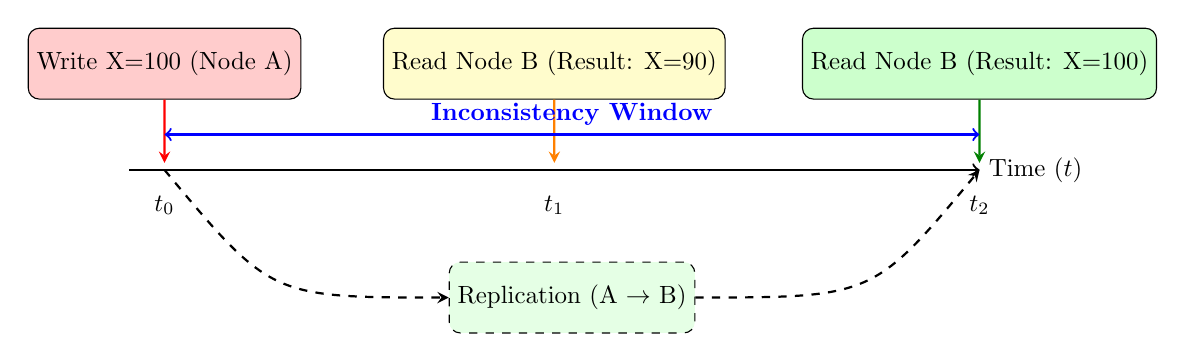
\begin{tikzpicture}[
        node distance=2cm,
        scale=0.9, transform shape,
        process/.style={rectangle, draw=black, fill=blue!10, rounded corners, minimum width=2.5cm, minimum height=1cm},
        arrow/.style={->, >=stealth, thick},
        timeline/.style={->, thick}
    ]

    % Time Axis
    \draw[timeline] (-2,0) -- (10,0) node[right] {Time ($t$)};
    
    % Events
    \node (write) at (-1.5, 1.5) [process, fill=red!20] {Write X=100 (Node A)};
    \draw[arrow, red] (write) -- (-1.5,0.1);
    \node at (-1.5, -0.5) {$t_0$};

    \node (read_fail) at (4, 1.5) [process, fill=yellow!20] {Read Node B (Result: X=90)};
    \draw[arrow, orange] (read_fail) -- (4,0.1);
    \node at (4, -0.5) {$t_1$};

    \node (sync) at (4.25, -1.8) [process, fill=green!10, dashed] {Replication (A $\rightarrow$ B)};
    \draw[arrow, dashed] (-1.5, 0) .. controls (0, -1.8) .. (sync.west);
    \draw[arrow, dashed] (sync.east) .. controls (8.5, -1.8) .. (10, 0);

    \node (read_success) at (10, 1.5) [process, fill=green!20] {Read Node B (Result: X=100)};
    \draw[arrow, green!50!black] (read_success) -- (10,0.1);
    \node at (10, -0.5) {$t_2$};

    % Annotations
    \draw[<->, thick, blue] (-1.5,0.5) -- (10,0.5) node[midway, above] {\textbf{Inconsistency Window}};

    \end{tikzpicture}
    \caption{Minh họa khoảng thời gian "Bất nhất quán" (Inconsistency Window) trong mô hình BASE. Mô hình Eventual Consistency: Dữ liệu tại Node B không cập nhật ngay lập tức nhưng sẽ nhất quán sau quá trình đồng bộ.}
    \label{fig:eventual_consistency}
\end{figure}

\paragraph{Sự chuyển dịch sang ACID trong NoSQL hiện đại}
Do nhu cầu nghiệp vụ phức tạp, ranh giới giữa SQL và NoSQL về transaction đang mờ dần.

\begin{figure}[H]
    \centering
    \begin{tikzpicture}[
        node distance=1cm,
        doc/.style={rectangle, draw=black, fill=white, drop shadow, minimum width=3.5cm, minimum height=4cm, align=left, font=\small\ttfamily},
        box/.style={rectangle, draw=red, dashed, thick, rounded corners, inner sep=10pt},
        arrow/.style={->, >=stealth, ultra thick, blue}
    ]

    \node[doc] (single) at (0,0) {
        \textbf{\{JSON: Order\}}\\
        \_id: 101\\
        total: \$500\\
        \textbf{items: [}\\
        \ \ \{sku: "A", qty: 1\},\\
        \ \ \{sku: "B", qty: 2\}\\
        \textbf{]}\\
        status: "NEW"
    };
    \node[above=1.75cm of single, font=\bfseries] {Single-Document (Embedded)};
    
    \draw[arrow] (-5, 0) -- node[above, font=\bfseries, text=black] {Atomic Update} (single.west);

    \node[doc, minimum height=1.5cm] (order) at (7, 1.5) {
        \textbf{\{Coll: Orders\}}\\
        \_id: 101\\
        status: "NEW"
    };
    
    \node[doc, minimum height=1.5cm] (stock) at (7, -1.5) {
        \textbf{\{Coll: Products\}}\\
        sku: "A"\\
        stock: 49
    };

    \node[above=1.5cm of order, font=\bfseries] {Multi-Document (Normalized)};

    \node[draw=green!50!black, thick, dashed, fit=(order) (stock), label=above:\textcolor{green!50!black}{\textbf{ACID Transaction Scope}}] (trans) {};

    \draw[arrow] (11.5, 0) -- node[above, font=\bfseries, text=black] {Transaction} (trans.east);
    \draw[->, thick] (trans.center) -- (order.south);
    \draw[->, thick] (trans.center) -- (stock.north);

    \end{tikzpicture}
    \caption{So sánh tính nguyên tử trên Single-Document (Mặc định) và Multi-Document Transaction}
    \label{fig:single_vs_multi_doc}
\end{figure}

\begin{itemize}[label=$\circ$]
    \item \textbf{Single-Document Atomicity:} Hầu hết NoSQL (Document, Key-Value) luôn đảm bảo tính nguyên tử trên một đơn vị dữ liệu duy nhất. Vì dữ liệu NoSQL thường được phi chuẩn hóa (Denormalized) và nhúng (Embedded), một thao tác ghi đơn lẻ thường giải quyết được 80-90\% nhu cầu nghiệp vụ mà không cần Multi-record Transaction.
    \item \textbf{Multi-Document ACID Transactions:} Các hệ thống NoSQL thế hệ mới (như MongoDB từ v4.0) đã hỗ trợ Transaction đa tài liệu với cơ chế tương tự SQL (Snapshot Isolation), cho phép cập nhật nhiều collection/shard một cách an toàn.
\end{itemize}

\subsubsection{SQL vs NoSQL}

Bảng dưới đây tổng hợp sự khác biệt cốt lõi về khả năng xử lý giao dịch giữa hai dòng cơ sở dữ liệu:

\begin{table}[H]
\centering
\renewcommand{\arraystretch}{1.4}
\begin{tabularx}{\textwidth}{|l|X|X|}
\hline
\textbf{Đặc điểm} & \textbf{SQL (Relational)} & \textbf{NoSQL (Non-Relational)} \\ \hline
\textbf{Triết lý thiết kế} & Tuân thủ chặt chẽ ACID. Dữ liệu được chuẩn hóa cao độ, yêu cầu transaction phức tạp để nối (JOIN) nhiều bảng. & Ưu tiên hiệu năng và mở rộng (BASE/CAP). Dữ liệu phi chuẩn hóa, ưu tiên atomic trên từng document/key. \\ \hline
\textbf{Phạm vi Transaction} & Hỗ trợ mạnh mẽ giao dịch phức tạp, kéo dài, bao trùm toàn bộ lược đồ cơ sở dữ liệu. & Thường tối ưu cho giao dịch cục bộ (single-shard/document). Giao dịch đa tài liệu (multi-document) có hỗ trợ nhưng ảnh hưởng hiệu năng. \\ \hline
\textbf{Cơ chế khóa (Locking)} & Sử dụng Row-level locking hoặc MVCC phức tạp để quản lý tranh chấp. & Thường sử dụng Optimistic Concurrency Control hoặc cấp phát khóa ở mức Document/Bucket. \\ \hline
\textbf{Xử lý phân tán} & Khó khăn hơn trong môi trường phân tán (cần 2PC gây độ trễ). & Thiết kế native cho phân tán (Sharding), nhưng transaction phân tán (Distributed Tx) rất tốn kém tài nguyên. \\ \hline
\end{tabularx}
\caption{So sánh đặc tính Transaction giữa SQL và NoSQL}
\label{tab:sql_nosql_trans}
\end{table}
